\documentclass[10pt, letterpaper]{article}

% --- Packages ---
\usepackage[margin=0.6in]{geometry}
\usepackage{booktabs}
\usepackage{tabularx}
\usepackage{enumitem}
\usepackage{titlesec}
\usepackage{mathpazo}
\usepackage[T1]{fontenc}
\usepackage{xcolor}
\usepackage{amsmath,amssymb}
\usepackage{graphicx}
\usepackage{hyperref}

% --- Color Definition ---
\definecolor{brandorange}{HTML}{F58025}

% --- Formatting Setup ---
\setlength{\parindent}{0pt}
\setlength{\parskip}{0.35em}

\titleformat{\section}{\bfseries\color{brandorange}}{}{0em}{}
\titlespacing{\section}{0pt}{0.6em}{0.15em}

\begin{document}

% --- Compact Header ---
{\large \textbf{Spectral Filtering for Sequential Decision Models}} \hfill \textbf{Team:} Shivam Kak, Ishan Saha, Connor Brown \\
\rule{\textwidth}{0.4pt}

% --- Abstract ---
\section*{Abstract}

Spectral Transfer Units (STUs) leverage Hankel matrix eigendecomposition for efficient long-range sequence modeling. We investigate their application to two sequential decision-making architectures. First, we integrate STU layers into the action prediction head of $\pi_{0.5}$, a vision-language-action (VLA) flow-matching model. On the LIBERO manipulation benchmark, STU-augmented models converge to within 7\% of the baseline training loss but do not improve over it, likely because the short action horizon ($H{=}10$) provides insufficient temporal structure for spectral filtering to exploit. Motivated by this negative result, we pivot to a setting with richer temporal structure: Transformer-based world models for model-based reinforcement learning. We propose augmenting the IRIS world model with STU layers to reduce compounding prediction errors during long-horizon imagined rollouts, where spectral filtering's global temporal modeling is better suited.

% --- Background ---
\section*{Background}

\textbf{Spectral Transfer Units.}
STUs~[1] convolve input sequences with spectral filters from the Hankel matrix $Z_{ij} = \frac{2}{(i+j)^3 - (i+j)}$. The top-$K$ eigenvectors $\phi_k$, scaled by the fourth root of their eigenvalues, serve as filters:
\begin{equation}
y = \textstyle\sum_{k=1}^{K} \left( (u * \phi_k^+) \cdot M_k^+ + (u * \phi_k^-) \cdot M_k^- \right)
\end{equation}
where $M_k^{\pm} \in \mathbb{R}^{D_{\text{in}} \times D_{\text{out}}}$ are learnable projections and convolution uses FFT in $O(L \log L)$ time. The connection to online control theory provides guarantees on approximating linear dynamical systems, suggesting STUs are well-suited for modeling structured temporal dynamics.

\textbf{VLA Models.}
The $\pi_0$ family~[2] combines a SigLIP vision encoder and PaliGemma language model with a lightweight action expert. In $\pi_{0.5}$, actions are predicted by denoising a noise vector via flow matching, producing a velocity field $v_t$ that guides $x_{t+dt} = x_t + dt \cdot v_t$.

\textbf{Transformer World Models.}
IRIS~[3] tokenizes observations via VQ-VAE and predicts next-frame tokens autoregressively with a GPT-like Transformer, achieving superhuman Atari 100k performance. However, small per-step prediction errors compound over long rollout horizons, degrading imagined trajectory quality. STORM~[4], TWISTER~[5], and TWM~[6] propose improvements but share this fundamental limitation.

% --- Part I: VLA Experiment ---
\section*{Experiment: STU-Augmented VLA Action Prediction}

\textbf{Method.}
We insert a residual STU block after the $\pi_{0.5}$ transformer action expert: given hidden states $h \in \mathbb{R}^{B \times H \times W}$, we apply $h' = h + \text{STU}(\text{LayerNorm}(h))$ before projecting to action space. The STU operates over the action horizon ($L = H = 10$). For the Gemma 300M action expert ($W = 1024$), STU-K4 adds $2 \times 4 \times 1024^2 \approx 8.4$M parameters (2.8\% overhead). All models fine-tune from the pre-trained $\pi_{0.5}$ checkpoint on LIBERO: AdamW (lr $= 5{\times}10^{-5}$), cosine decay, batch size 8, 5000 steps on a single A100 80GB.

\textbf{Results.}
Figure~\ref{fig:loss} and Table~\ref{tab:results} summarize training. Neither STU variant improves over the baseline: both converge to loss 0.031 vs.\ the baseline's 0.029. STU models start with higher loss due to randomly initialized spectral projections but recover by step ${\sim}2000$. K4 and K8 reach identical final loss despite K8 having twice the parameters, and neither adds wall-clock overhead.

\begin{figure}[h]
\centering
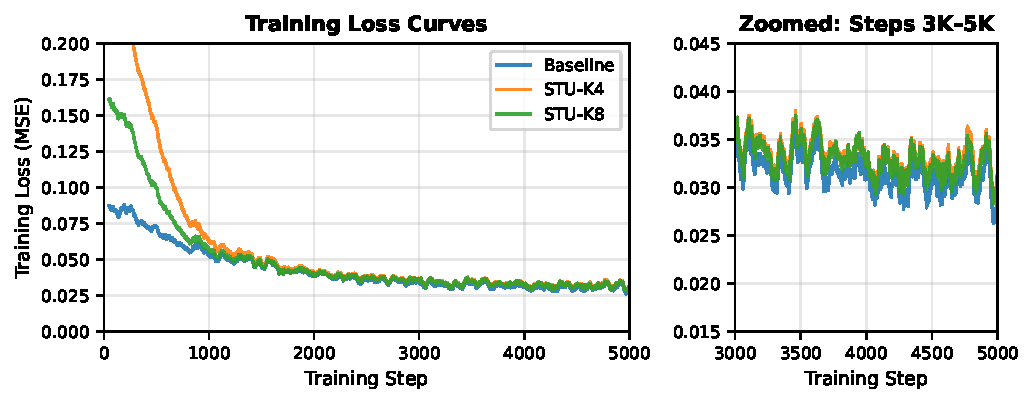
\includegraphics[width=\linewidth]{loss_curves.pdf}
\caption{Training loss (50-step rolling average). STU variants start higher but converge to near-baseline by step $\sim$2000. Zoomed view (right) shows all three models are nearly indistinguishable in the final 2000 steps.}
\label{fig:loss}
\end{figure}

\begin{table}[h]
\centering
\small
\begin{tabular}{@{}lcccc@{}}
\toprule
\textbf{Model} & \textbf{Final Loss} & \textbf{Init Loss} & \textbf{Extra Params} & \textbf{s/step} \\
\midrule
Baseline & \textbf{0.029} & 0.070 & 0 & 1.53 \\
STU-K4   & 0.031 & 0.141 & 8.4M (2.8\%) & 1.48 \\
STU-K8   & 0.031 & 0.101 & 16.8M (5.6\%) & 1.54 \\
\bottomrule
\end{tabular}
\caption{VLA training results. Final loss averaged over last 100 steps. Both STU variants converge to within 7\% of baseline.}
\label{tab:results}
\end{table}

\textbf{Analysis.}
LIBERO's short action horizon ($H{=}10$) likely provides insufficient temporal structure for spectral filtering. With only 10 timesteps, even $K{=}4$ filters oversaturate the sequence, and the transformer already has sufficient capacity. The residual connection allows the model to effectively bypass the STU block, recovering near-baseline behavior. This motivates applying STUs to a setting with longer sequences and more temporal structure.

% --- Part II: Proposed Direction ---
\section*{Proposed Direction: STU-Augmented World Models}

\textbf{Motivation.}
Unlike VLA action prediction over 10 timesteps, world models generate imagined rollouts over tens to hundreds of steps. Each autoregressive prediction introduces small errors that compound, shifting the state distribution away from training data. STUs' global spectral filtering is better matched to this longer-horizon setting: the spectral filters encode low-frequency trends and periodic patterns that local attention must learn implicitly. Game environments exhibit structured temporal patterns (periodic spawns, predictable physics) that spectral filters can efficiently capture.

\textbf{Architecture.}
We propose two integration strategies for the IRIS dynamics backbone: (1)~\textbf{Residual STU blocks} between Transformer layers, where attention captures local token dependencies and STU captures global temporal patterns; (2)~\textbf{STU dynamics head}, replacing the Transformer entirely to test whether spectral filtering alone suffices. The discrete autoencoder and actor-critic policy remain unchanged.

\textbf{Planned Experiments.}
We will evaluate on Atari 100k~[7] following the IRIS protocol (5 seeds, 100k environment steps). Key metrics beyond standard human-normalized scores: (1)~\textit{Rollout fidelity vs.\ horizon}---condition on $C$ real frames and measure prediction error at $H \in \{5, 10, 15, 25, 50\}$ to directly quantify compounding error; (2)~\textit{Performance per parameter}---comparing parameter efficiency of STU vs.\ Transformer dynamics; (3)~\textit{Imagination horizon sensitivity}---if STUs reduce compounding error, longer horizons should benefit STU models more. Baselines include IRIS (Transformer backbone) with ablations over $K \in \{4, 8, 16, 32\}$ spectral filters.

% --- References ---
\section*{References}
\begin{enumerate}[leftmargin=1.5em, nosep, label={[\arabic*]}]
    \item Agarwal, N., Hazan, E., et al. Spectral State Space Models. \textit{arXiv:2312.06837}, 2023.
    \item Physical Intelligence. $\pi_0$: A Vision-Language-Action Flow Model for General Robot Control. \textit{arXiv:2410.24164}, 2024.
    \item Micheli, V., Alonso, E., Fleuret, F. Transformers are Sample-Efficient World Models. \textit{ICLR}, 2023.
    \item Zhang, W., et al. STORM: Efficient Stochastic Transformer based World Models. \textit{NeurIPS}, 2023.
    \item Patalay, A., et al. TWISTER: Transformer WIth State-action rEpResentation. \textit{Preprint}, 2024.
    \item Robine, J., et al. Transformer-based World Models Are Happy With 100k Interactions. \textit{ICLR}, 2023.
    \item Kaiser, L., et al. Model Based Reinforcement Learning for Atari. \textit{ICLR}, 2020.
\end{enumerate}

\end{document}
